% XXX: fix hard-coded fig nums
\chapter{Spin-orbit protection of induced superconductivity in Majorana nanowires}
\label{ch:spinorbit}

%% Start the actual chapter on a new page.
\newpage
\noindent
\section{Introduction}

Spin-orbit interaction (SOI) is a relativistic effect that results from electrons moving (orbit) in an electric field ($E$) experiencing a magnetic field ($B_{\mathrm{SO}}$) in their moving reference frame that couples to the electron's magnetic moment (spin).
SOI is an essential ingredient of various realizations of topological superconductors, which host Majorana zero modes, the building blocks of topological quantum computation \cite{Kitaev2001,Fu2008,Nayak2008}.
The prime platform for topological quantum computation is based on a semiconductor nanowire coupled to a superconductor, where the proximity effect opens a superconducting energy gap in the density of states of the nanowire \cite{Lutchyn2010,Oreg2010}.
In general, a magnetic field suppresses superconductivity by closing the superconducting gap due to Zeeman and orbital effects \cite{Nijholt2016}.
If the nanowire has strong SOI, suppression of the superconducting gap is counteracted and a sufficiently large Zeeman energy drives the system into a topological superconducting phase, with Majorana zero modes localized at the wire ends \cite{Lutchyn2010,Oreg2010}.
The main experimental effort in the last few years has focused on detecting these Majorana zero modes as a zero-bias peak in the tunneling conductance \cite{Mourik2012,Albrecht2016,Deng2016,BalMaj,QZBP,LutchynReview,AguadoReview}.
However, SOI, the mechanism providing the topological protection, has been challenging to detect directly in Majorana nanowires.

The electric field that gives rise to SOI in our system mainly results from structural inversion asymmetry of the confinement potential (Rashba SOI), which depends on the work function difference at the interface between the nanowire and the superconductor and on voltages applied to nearby electrostatic gates \cite{Vuik2016,Antipov2018,Woods2018,Mikkelsen2018}.
The Rashba SOI in nanowires has been investigated extensively by measuring spin-orbit related quantum effects: level repulsion of quantum dot levels \cite{Fasth2007,NadjPerge2012}, and of Andreev states \cite{DeMoor2018,Deng2016}, weak antilocalization in long \mbox{diffusive} wires \cite{Hansen2005,VanWeperen2015}, and a helical liquid signature in short quasiballistic wires \cite{JakobHelical}.
However, the SOI strength relevant to the topological protection is affected by the \mbox{presence} of the superconductor, necessitating direct observation of SOI in Majorana nanowires.
Here, we reveal SOI in an InSb nanowire coupled to a NbTiN superconductor through the dependence of the superconducting gap on the magnetic field, both strength and orientation.
We find that the geometry of the superconductor on the nanowire strongly modifies the direction of the spin-orbit field, which is further tunable by electrostatic gating, in line with the expected modifications of the electric field due to work function difference and electrostatic screening at the nanowire-superconductor interface.

Figure 1(a) shows the device image.
An InSb nanowire (blue) is covered by a NbTi/NbTiN superconducting contact (purple) and a Cr/Au normal metal contact (yellow).
The barrier gate underneath the uncovered wire (red) can deplete the nanowire, locally creating a tunnel barrier.
The tunneling differential conductance ($dI/dV$) resolves the induced superconducting gap, by sweeping the bias voltage ($V$) across the tunnel barrier [Fig. 1(b)].
The dashed arrow indicates the induced gap of 0.65 meV.
In this device, we have recently shown ballistic transport and Majorana signatures \cite{BalMaj}.
\begin{figure}
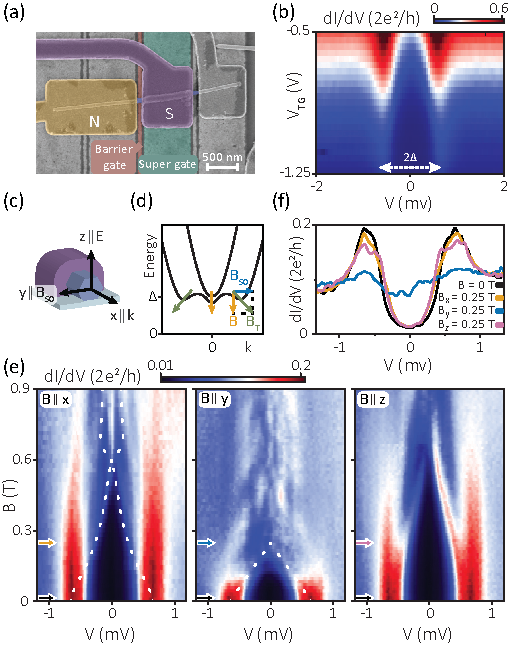
\includegraphics[width=\columnwidth]{chapter_spinorbit/figures/Fig1.pdf}
\caption{\label{fig:fig1}
(a) False-color scanning electron micrograph of Majorana nanowire device $A$.
An InSb nanowire (blue) is contacted by a normal metal contact ($N$, yellow) and a NbTiN superconducting contact ($S$, purple).
The additional contact (gray) is kept floating.
The nanowire is isolated from the barrier gate (red) and the super gate (green) by $\sim$ 30 nm thick boron nitride.
(b) Differential conductance $dI/dV$ as a function of bias voltage $V$ and barrier gate voltage $V_{\mathrm{barrier}}$ at $B$ $=$ 0 T.
(c) Schematic of the nanowire device and definition of the axes.
(d) Band diagram of a Majorana nanowire at an externally applied magnetic field $B$ perpendicular to the spin-orbit field $B_{\mathrm{SO}}$.
The arrows indicate the total magnetic field $B_T$ $=$ $B$ + $B_{\mathrm{SO}}$ along which the spin eigenstates are directed.
At $k$ $=$ 0 the spin always aligns with $B$.
At increasing $k$, $B_{\mathrm{SO}}$ increases, tilting the spin more towards $B_{\mathrm{SO}}$.
(e) $dI/dV$ as a function of $V$ at $B$ along $x$, $y$, $z$ (left, middle, right) for super gate voltage $V_{\mathrm{SG}}$ $=$ 0 V.
The white dashed lines indicate a fit to the gap closing corresponding to $\alpha$ $=$ 0.15 $\pm$ 0.05 eV\AA.
(f) Horizontal line cuts of (e) at $B$ indicated by the colored arrows in (e).
}
\end{figure}

The magnetic field ($B$) dependence of the induced gap of device $A$, with $B$ along three different directions, is shown in Fig. 1(e).
The coordinate system is illustrated in Fig. 1(c).
The $x$ axis is along the nanowire, parallel to the electron momentum ($k$).
The $z$ axis is perpendicular to the substrate and coincides with the electric field ($E$) direction due to the spatial symmetry of the device and the bottom gate.
Since the Rashba spin-orbit field ($B_{\mathrm{SO}}$ $\propto$ $E$ $\times$ $k$) is perpendicular to both $k$ and $E$, it points along the $y$ axis.
When $B$ is aligned with $x$ or $z$ [left and right panels in Fig. 1(e)], both perpendicular to $B_{\mathrm{SO}}$, the gap closes \mbox{slowly} (at around 0.6 T), followed by the emergence of a zero-bias peak possibly characteristic of a Majorana zero mode when $B$ is along the nanowire, although we emphasize that a conjecture of Majorana zero modes is not essential for the purposes of this chapter.
On the contrary, when $B$ is aligned with the $y$ axis (middle panel), parallel to $B_{\mathrm{SO}}$, the gap closes much faster (at around 0.25 T).
Figure 1f shows the line cuts at $|B|$ $=$ 0.25 T along the three axes: for $B$ $\perp$ $B_{\mathrm{SO}}$, the gap is almost the same as when $B$ $=$ 0 T, while the gap is closed for $B$ $\parallel$ $B_{\mathrm{SO}}$.
This observation matches the predictions of the Majorana nanowire model, as illustrated in Fig. 1(d): when $B$ $\perp$ $B_{\mathrm{SO}}$, SOI counteracts the Zeeman-induced gap closing by rotating the spin eigenstate towards $B_{\mathrm{SO}}$, which reduces the component of the Zeeman field along the direction of the spin eigenstate.
In contrast, when $B$ $\parallel$ $B_{\mathrm{SO}}$, the spin eigenstate is always parallel to $B$, which prevents spin-orbit protection and results in a fast gap closing \cite{Osca2014,Rex2014}.
This pronounced anisotropy of the gap closing with respect to different $B$ directions is universally observed in over ten devices (four shown in this chapter) for all gate settings
\footnote{See Supplemental Material, which includes Refs.
 \cite{Car2014,Flohr2011,Suyatin2007,HardGap,Liu2017,Danon2017,Hofstader1976,Gropp1996,Du1999,Prada2012,Pientka2012,Stanescu2012}, for experimental details, theoretical details, and additional experimental data}, which is a direct consequence of SOI in Majorana nanowires.
\nocite{Car2014,Flohr2011,Suyatin2007,HardGap,Liu2017,Danon2017,Hofstader1976,Gropp1996,Du1999,Prada2012,Pientka2012,Stanescu2012}

Before we discuss the SOI in more detail, we rule out alternative mechanisms for the anisotropy which can originate in the bulk superconductor, or the InSb nanowire.
First, an anisotropic magnetic field-induced closing of the bulk superconducting gap is excluded for the fields we apply, which are far below the critical field of NbTiN ($>$9 T) \cite{DavidOneMin}.
We note that this is different from aluminium films \cite{Chang2015,Deng2016,Gazibegovic2017,QZBP}, where a small magnetic field ($<$0.3 T) perpendicular to the film completely suppresses superconductivity, making them unsuitable to reveal SOI from an anisotropic gap closing.
Next, we consider Meissner screening currents in NbTiN that can cause deviations in the magnetic field in the nanowire.
Our Ginzburg-Landau simulations show that the field corrections due to Meissner screening are negligible \cite{Note1}, since the dimensions of the NbTiN film ($<$1 $\mu$m) are comparable to the penetration depth ($\sim$290 nm).  % XXX: fix Note1
The simulations also show that vortex formation is most favorable along the $z$ axis \cite{Note1}, which implies that the observed anisotropic gap closing is not caused by gap suppression due to vortices near the nanowire \cite{Takei2013}, since we do not observe the fastest gap closing along $z$ [Fig. 1(f)].  % XXX: fix Note1
Finally, in the InSb nanowire, the Zeeman $g$ factor can become anisotropic due to quantum confinement \cite{NadjPerge2012,Pryor2006,Qu2016}.
However, our nanowire geometry leads to confinement in both the $y$ and $z$ directions, implying similar gap closing along $y$ and $z$, inconsistent with our observations [Fig. 1(e)].

Having excluded the above mechanisms, we are now left with three effects: spin splitting of the electron \mbox{states} in magnetic fields with the Land\'e $g$ factor (Zeeman eff\mbox{ect)}, the orbital effect of the magnetic field representing the Lorentz force acting on traveling electrons, and SOI.
To investigate the role of these effects, we use a theoretical three-dimensional Majorana nanowire model defined by the Hamiltonian \cite{Lutchyn2010,Oreg2010,Nijholt2016}:
\begin{equation*}
\begin{split}
H = &\left(\frac{\mathbf{p}^2}{2m^*}-\mu+V(y,z)\right) \tau_z + \frac{\alpha}{\hbar} \boldsymbol{\sigma} \cdot \mathbf{(\hat{E}\times p)} \tau_z\\
&+ \frac{1}{2}g\mu_B\mathbf{B\cdot}\boldsymbol{\sigma}+\Delta_0 \tau_x
\end{split}
\end{equation*}
Here, the first term represents the kinetic and potential energy, with $\mu$ the chemical potential measured from the middle of the helical gap and $V(y,z)$ $=$ $\frac{\Delta V_G}{R}[0,y,z]$ $\cdot$ $\mathbf{\hat{E}}$ is the electrostatic potential in the wire, whose magnitude is parametrized by $\Delta V_G$, with $\mathbf{\hat{E}}$ the direction of the electric field and $R$ the wire radius.
The orbital effect enters the Hamiltonian via the vector potential $\mathbf{A}$ in the canonical momentum: $\mathbf{p}$ $=$ $-i\hbar \nabla$ $+$ $e\mathbf{A}$.
Here, $e$ is the electron charge, $\hbar$ is Plank's constant, and $m^*$ $=$ 0.015 $m_e$ is the effective mass with $m_e$ the electron mass.
The second term represents Rashba SOI characterized by a SOI strength $\alpha$, which we set to 0.2 eV\AA\ to find qualitative agreement with the measurements.
The third term is the Zeeman term, with an isotropic $g$ factor set to 50 and $\mu_B$ is the Bohr magneton.
The last term accounts for the superconducting proximity effect, which we implement in the weak coupling approximation \cite{Nijholt2016}.
The Pauli matrices $\tau$ and $\sigma$ act in the particle-hole and spin space respectively.
We perform numerical simulations of this Hamiltonian on a 3D lattice in a realistic nanowire geometry using the \textsc{kwant} code \cite{Groth2014}.
We note that recent theory work shows that the anisotropy is unaffected by additional factors such as the wire length, temperature, and strong coupling to the superconductor \cite{Liu2019}.
Additional details are provided in the Supplemental Material \cite{Note1}.  % XXX: fix Note1
\begin{figure}
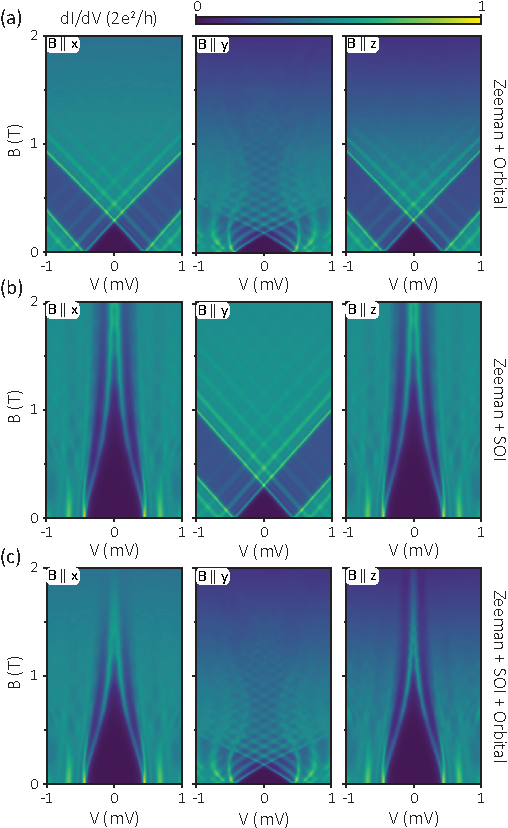
\includegraphics[width=\columnwidth]{chapter_spinorbit/figures/Fig2.pdf}
\caption{\label{fig:fig2}
(a) Numerical simulations of $dI/dV$ as a function of $V$ and $B$, including the Zeeman and the orbital (Lorentz) effect of the magnetic field.
(b) Same as (a), but including Zeeman and SOI instead of the orbital effect, reproducing the anisotropy in Fig. 1(e).
(c) Same as (b), but including the Zeeman, SOI and orbital effect.
The parameters used in (a)-(c) are $\mu$ $=$ 5.6 meV and $\Delta V_G$ $=$ -8 meV.
}
\end{figure}

We identify which effects explain the observed anisotropic gap closing behavior by including them separately in our simulations.
Figure 2(a) shows the magnetic field dependence of the gap without SOI (setting $\alpha$ $=$ 0 in the Hamiltonian).
In contrast to Fig. 1(e) the gap closes around 0.3 T for all three directions, reflecting the dominant contribution of the Zeeman effect.
In Fig. 2(b), we turn on the SOI, and turn off the orbital effect by setting the magnetic vector potential $\mathbf{A}$ $=$ 0, which qualitatively reproduces the anisotropic behavior between the $y$ axis and the $x$ and $z$-axes.
We have explored other combinations of parameters and find that the experimental results of Fig. 1(e) can only be reproduced by including SOI.
We note that adding the orbital effect in Fig. 2(c) shifts the gap closing to a field almost twice as small for $B$ $\parallel$ $y$, which explains why we observe a gap closing for $B$ $\parallel$ $y$ at around 0.25 T, far below 0.45 T, the critical field expected when only the Zeeman effect with $g$ $=$ 50 suppresses the gap.
By fitting the curvature of the gap closing \cite{VanHeck,Pan2018} along $x$ [white dashed line in Fig. 1(e)] we estimate a range of the SOI strength $\alpha$ of 0.15 -- 0.35 eV\AA\ from devices $A$-$D$ (for fitting details and fits to additional devices, see Supplemental Material \cite{Note1}).  % XXX: fix Note1
This SOI strength is in \mbox{agreement} with the values extracted from level repulsion of Andreev states \cite{Stanescu2013,DeMoor2018} in an additional device $E$ \cite{Note1}.  % XXX: fix Note1
\mbox{Since} $\alpha$ depends on the electric field in the wire, we expect the observed variation in the SOI strength of devices to be caused by differences in the applied gate voltages and wire diameter.
Recently, the level repulsion of Andreev states in InSb nanowires covered with epitaxial aluminium has shown a SOI strength of approximately 0.1 eV\AA \cite{DeMoor2018}, slightly lower than we find for NbTiN covered nanowires, most likely due to strong coupling to the aluminium superconductor, leading to stronger renormalization of the InSb material parameters \cite{Stanescu2011,Cole2015,Antipov2018,Woods2018,Mikkelsen2018,Reeg2018}.
\begin{figure}
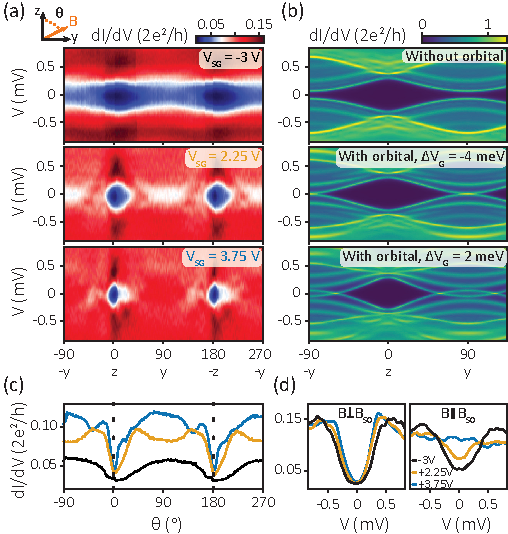
\includegraphics[width=\columnwidth]{chapter_spinorbit/figures/Fig3.pdf}
\caption{\label{fig:fig3}
(a) Measured $dI/dV$ as a function of $V$ upon rotation of $B$ at 0.3 T over angles $\Theta$ between $z$ and $y$ in device $B$ (see Fig. S5 \cite{Note1} for the same behavior in device $A$).  % XXX: fix Note1
The voltage $V_{\mathrm{SG}}$ on the super gate (see insets) is varied in the three panels.
(b) Simulated $dI/dV$ as a function of $\Theta$ and $V$ at 0.25 T.
The top panel includes the Zeeman effect and SOI.
The middle and bottom panels additionally include the orbital effect at two values of the potential difference $\Delta V_G$ between the top and middle of the wire.
(c) Horizontal line cuts of (a) averaged over $|V|$ $<$ 0.2 V at $V_{\mathrm{SG}}$ $=$ -3,  2.25, and 3.75 V (black, orange, blue).
Dashed lines indicate the $z$ axis ($\Theta$ $=$ \ang{0}).
(d) Vertical line cuts of (a) at $\Theta$ $=$ \ang{0} (left) and $\Theta$ $=$ \ang{90} (right).
}
\end{figure}

To resolve the direction of the spin-orbit field, we fix the $B$ amplitude and continuously rotate the $B$ direction, parametrized by the angle $\Theta$ in the $zy$ plane [inset Fig. 3(a)].
Figure 3(a) shows the dependence of the gap on $\Theta$, where we adjust the electric field strength in the nanowire with a voltage $V_{\mathrm{SG}}$ on the super gate (SG) underneath the superconductor [green in Fig. 1(a)].
We define the angle at which the gap is hardest as $\Theta_{\mathrm{max}}$ and find $\Theta_{\mathrm{max}}$ $=$ 3 $\pm$ \ang{2} ($z$ axis) for all $V_{\mathrm{SG}}$ and in multiple devices (Fig. 3 and Fig. S5 \cite{Note1}) (error due to uncertainty in the extraction procedure).  % XXX: fix Note1
This is illustrated in Fig. 3(c), which shows horizontal line cuts for subgap bias.
The largest gap for a given $B$ amplitude is expected for $B$ $\perp$ $B_{\mathrm{SO}}$, indicating that $B_{\mathrm{SO}}$ $\parallel$ $y$, in agreement with the $E$-field direction dictated by the device geometry.

\begin{figure}[b]
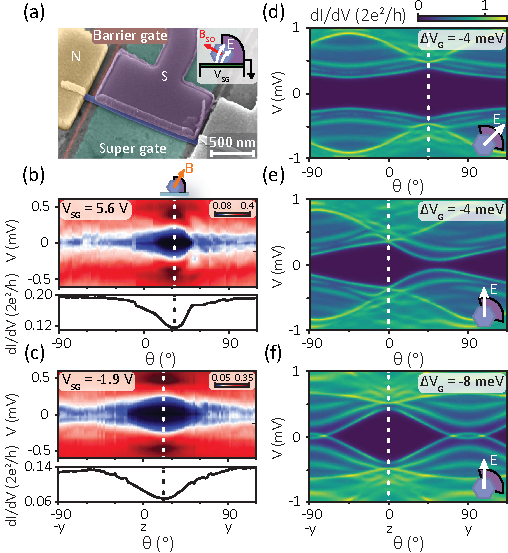
\includegraphics[width=\columnwidth]{chapter_spinorbit/figures/Fig4.pdf}
\caption{\label{fig:fig4}
(a) Tilted view electron micrograph of Majorana nanowire device $E$, which is partially covered with NbTiN.
In this device, the electric field $E$ (and the associated spin-orbit field $B_{\mathrm{SO}}$) can rotate away from the $z$ axis ($y$ axis), as illustrated in the inset.
(b) Measured $dI/dV$ as a function of $V$ and angle $\Theta$ in the $zy$ plane at $|B|$ $=$ 75 mT and $V_{\mathrm{SG}}$ $=$ 5.6 V, with a horizontal line cut averaged over $|V|$ $<$ 0.25 mV in the lower panel.
The gap is maximum at $\Theta_{\mathrm{max}}$ $=$ \ang{32} as indicated by the dashed line.
(c) Same as (b), but at $V_{\mathrm{SG}}$ $=$ -1.9 V and $|B|$ $=$ 0.15 T.
$\Theta_{\mathrm{max}}$ is gate tuned to \ang{22}.
(d)-(f) Simulated $dI/dV$ at 0.25 T at various $\Delta V_G$ (see inset) with the superconductor rotated to the side by \ang{45} and including the Zeeman effect, SOI, and the orbital effect.
The illustrations in the insets indicate the direction of $E$, which is rotated by \ang{45} from $z$ in (d).
}
\end{figure}

Now, we check whether the orbital effect changes $\Theta_{\mathrm{max}}$.
The simulations in Fig. 3(b) show the effect of magnetic field rotation on the gap with $B_{\mathrm{SO}}$ $\parallel$ $y$, confirming that $\Theta_{\mathrm{max}}$ is, indeed, always given by the direction perpendicular to $B_{\mathrm{SO}}$, i.e.
$\Theta_{\mathrm{max}}$ $=$ \ang{0}.
Comparing the top panel (without the orbital effect) with the middle panel (with the orbital effect), we conclude that the orbital effect does not affect $\Theta_{\mathrm{max}}$.
This conclusion also holds when we vary the potential difference $\Delta V_G$ between the middle and outer of the wire (corresponding to $V_{\mathrm{SG}}$) in the middle panel and bottom panel.
We note that, at $\Delta V_G$ $=$ 2 meV (bottom panel) the wave function is moved towards the bottom of the nanowire, which increases the strength of the orbital effect by breaking the reflection symmetry about the $z$ axis, as evidenced by the longer angle range over which the gap is closed compared to $\Delta V_G$ $=$ -4 meV (middle panel).
Experimentally, we also observe this in Fig. 3(a), with line cuts in Fig. 3(c), where the gap is closed over a significantly longer angle range with increasing $V_{\mathrm{SG}}$.
We note that we use small values of $\Delta V_G$ in the simulations, because we expect a weak gate response due to effective electrostatic screening by the superconductor, which covers five of the six nanowire facets \cite{BalSc}.

Finally, we turn to a second type of device in which the superconducting film only partially covers the nanowire facets [Fig. 4(a)].
This partial superconductor coverage can modify the orientation of $B_{\mathrm{SO}}$ by changing the associated electric field direction \cite{Vuik2016}, as sketched in the inset of Fig. 4(a).
The electric field in the wire has two main origins.
The first one originates from the work function difference between the superconductor and nanowire, which leads to charge redistribution.
The resulting electric field is expected to rotate away from the $z$ axis due to the partial superconductor coverage which breaks the spatial symmetry.
In Fig. 4(b) we rotate $B$ in the $zy$ plane, perpendicular to the nanowire axis, and find that $\Theta_{\mathrm{max}}$ is, indeed, no longer at zero, but at 32 $\pm$ \ang{2}.
The second contribution to the electric field arises from the applied $V_{\mathrm{SG}}$ and the electrostatic screening due to the grounded superconductor.
Changing $V_{\mathrm{SG}}$ should, therefore, rotate the electric field for partial coverage.
Indeed, we find that $\Theta_{\mathrm{max}}$ shifts by \ang{10} by adjusting $V_{\mathrm{SG}}$ by 7.5 V [Fig. 4(c)].
Field rotation at intermediate $V_{\mathrm{SG}}$ and magnetic field sweeps confirming the change of $\Theta_{\mathrm{max}}$ are shown in the Supplemental Material \cite{Note1}.  % XXX: fix Note1
Our theory simulations confirm that $\Theta_{\mathrm{max}}$ is still given by the direction orthogonal to $B_{\mathrm{SO}}$ when the electric field is not necessarily along a \mbox{spatial} symmetry axis of the partially covered device [Fig. 4(d) and 4(e)].
While the orbital effect does not change $\Theta_{\mathrm{max}}$ [Fig. 4(e) and 4(f)], it can induce asymmetry in the energy spectrum around $\Theta_{\mathrm{max}}$ resulting from wave function asymmetry when the electric field is not along the mirror plane of the device [Fig. 4(b) and Fig. 4(e)].
The significance of the orbital effect in our devices underlines the importance of including it in realistic simulations of Majorana nanowires.

In conclusion, the observed gap closing anisotropy for different magnetic field orientations demonstrates SOI in our Majorana nanowires, a necessary condition to create Majorana zero modes.
Our experiments reveal that SOI is strongly affected by the work function difference at the nanowire-superconductor interface and the geometry of the superconductor, while electrostatic gating provides tunability of SOI.

\section{Appendix}

\subsection{Supplemental Experimental Details}
\subsubsection{Nanowire growth and device fabrication}
The \mbox{InSb} nanowires used here were grown using a Au-catalysed vapor-liquid-solid mechanism in a metal organic vapor phase epitaxy reactor, resulting in zinc blende nanowires grown \mbox{along} the [111] crystal orientation, which are free of stacking \mbox{faults} and dislocations \cite{Car2014}.
Local gates, covered by a h-BN dielectric flake, were fabricated on a silicon substrate.
The nanowires were individually placed over the gates using a micromanipulator \cite{Flohr2011}.
The contacts are fabricated by exposing the chip to a mild oxygen plasma cleaning after resist development, followed by immersion in a saturated ammonium polysulphide solution diluted by water to a 1:200 ratio for 30 minutes at \ang{60}C \cite{Suyatin2007}.
For the normal contacts, the wires are exposed to 30 seconds of in-situ helium ion milling, before evaporating 10 nm Cr and 110 nm Au.
The NbTiN contacts are fabricated by exposing the nanowire to 5 seconds or Ar plasma etching at 25 W, followed by sputtering of 5 nm NbTi and 85 nm NbTiN \cite{HardGap,BalSc}.

\subsubsection{Measurement details}
The measurements were performed in a dilution refrigerator at an electron temperature of $\sim$ 50 mK  using a three-axis vector magnet and standard lockin techniques.

\subsection{Supplemental Theoretical Details}
\subsubsection{Details of the tight binding simulations}
The Hamiltonian defined in the main text is discretized on a lattice of a realistic nanowire geometry with a diameter of 70 nm and a length of 2 $\mu$m using a lattice spacing of 10 nm.
The nanowire is covered by a 35 nm thick superconducting shell covering 3/8 of the circumference of the wire, posititioned on top of the wire [Fig.~2, 3(b)] or rotated from the top to the side by \ang{45} [Fig.~4(b)].
Transport calculations are performed by connecting the nanowire to semi-infinite normal leads, separated by a tunnel barrier on one side.
The normal leads provide broadening of the peaks in the simulations \cite{Liu2017,Danon2017}.
The superconducting proximity effect is implemented using the weak coupling approximation \cite{Nijholt2016}, in which the pairing gap $\Delta_0$ $=$ 0 in the nanowire, which is tunnel coupled to a superconductor with $\Delta_0$ $>$ 0 providing an induced gap of 0.45 meV at $B$ $=$ 0 T.
The potential in the wire is given by $V(y,z)= \frac{\Delta V_G}{R} (z\cos(\Phi)+y\sin(\Phi))$, where $\Delta V_G$ is the potential difference between the middle and outer points of the wire, $R$ is the radius of the nanowire, and $\Phi$ parametrizes the direction of the electric field $\mathbf{\hat{E}}$, which is set to $\Phi$ = \ang{0} in all simulations, except for Fig.~4(d), where $\Phi$ = \ang{45}.
The vector potential $\mathbf{A} = \left[B_y(z-z_0)-B_z(y-y_0),0,B_x(y-y_0)\right]^T$ is chosen such that it does not depend on $x$ and the offsets $x_0$, $y_0$, $z_0$ are chosen such that the vector potential averages to zero inside the superconductor, implying a total supercurrent of zero in the superconductor.
This choice is supported by the negligible screening currents we observe in our Ginzburg-Landau simulations [Fig.~\ref{fig:GL}].
$\mathbf{A}$ is implemented in the tight-binding model by Peierls substitution in the hopping amplitudes \cite{Hofstader1976}.

\subsubsection{Details of the Ginzburg-Landau simulations}
To calculate the stray fields in the nanowire due to Meissner screening and vortex entry in the superconducting contact (results shown in Fig.~\ref{fig:GL}), we have performed simulations on the Ginzburg-Landau model \cite{Gropp1996} in a realistic three-dimensional geometry using the dimensions of device A.
We used a penetration depth $\lambda$ = 290 nm and a Ginzburg-Landau parameter $\kappa = \lambda / \xi$ = 50, in line with the values expected for our NbTiN film, which has a room temperature resistivity of 95 $\mu \Omega$cm and a critical temperature of 15 K.
The Ginzburg-Landau functional is discretized both inside the superconducting contact as well as in its surrounding space \cite{Du1999} using a second-order finite difference scheme at a maximum internode distance of 0.01$\lambda$.
The resulting energy functional is minimized using the nonlinear conjugate gradient method and the code is implemented on a NVidia CUDA architecture with high parallelization.
We obtain the energy of states with vortices at finite magnetic fields by first introducing artificial perturbations near the sample boundary, followed by energy minimization to find the local minimum corresponding to a specific number of vortices.
The optimal number of vortices at a certain magnetic field is then determined by finding the state with the lowest energy globally.
We note that non-optimal amounts of vortices can be metastable due to significant Bean-Livingston barriers for vortex entry, so the actual number of vortices is hysteretic and depends on the dynamics of the magnetic field.

\begin{figure}
\centering
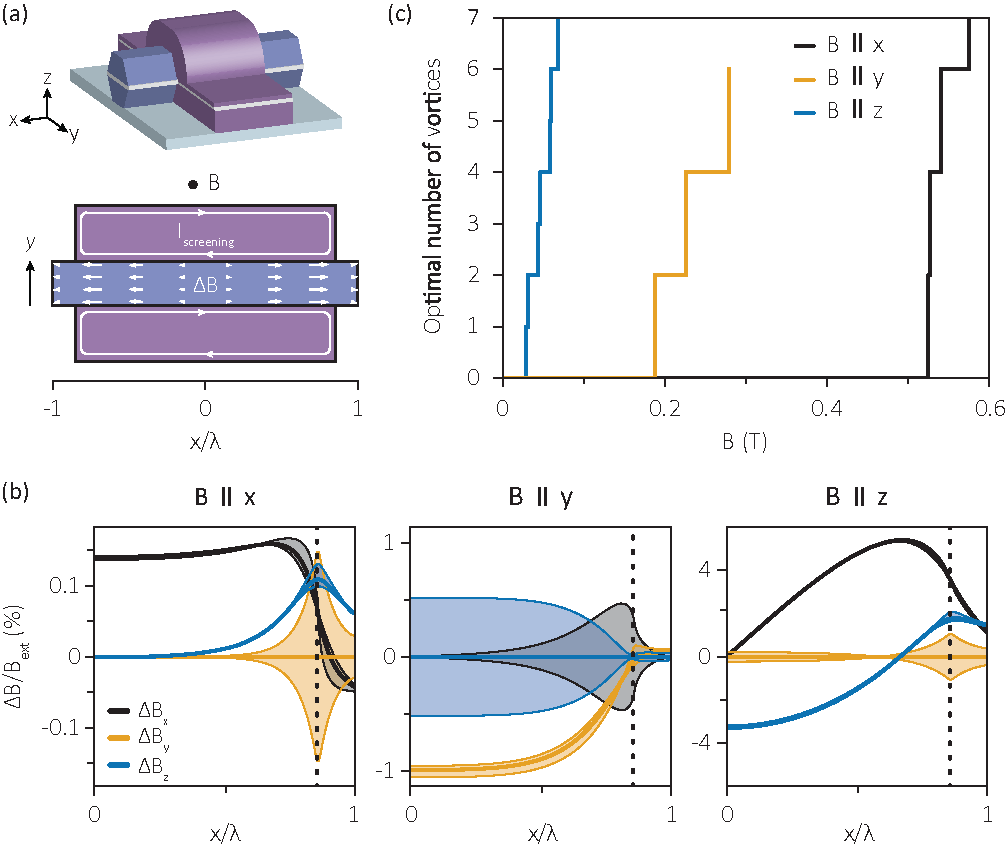
\includegraphics[width=0.95\textwidth]{chapter_spinorbit/figures/SFig2_GL.pdf}
\caption{\label{fig:GL}
Ginzburg-Landau simulations.
(a) The top panel shows the schematic of the geometry used for Ginzburg-Landau simulations: a superconducting film covering a hexagonal nanowire.
In a superconductor exposed to an external magnetic field $B$ we calculate the screening currents $I_{\mathrm{screening}}$, which induce stray magnetic fields $\Delta B$ in the nanowire.
In (b) we show $\Delta B$ in the $xy$-plane in the middle of the nanowire, as indicated by the white line in (a).
The bottom panel shows a top view of this $xy$-plane, where the arrows indicate the $x$ and $y$ components of $\Delta B$ in the nanowire for $B \parallel z$.
(b) The $x$, $y$ and $z$-components (black, yellow, blue) of $\Delta B$ relative to the external field $B$ as a function of the position $x$ along the nanowire axis, where $x = 0$ corresponds to the middle of the superconducting contact.
The lines show the mean stray field and the shaded regions are bounded by the minimum and maximum stray field found along the nanowire width at a particular $x$.
 The end of the superconducting film is indicated by the dashed line.
 $B$ is along $x$, $y$ and $z$ (left, middle and right panel).
Since the device dimensions are comparable to the penetration depth $\lambda = 290$ nm, the magnetic screening in the superconductor is incomplete, leading to small screening currents and stray fields of at most 4\% of $B$.
These modifications are much smaller and do not match the anisotropy we observe in the measurements, which excludes Meissner screening as the origin of the observed anisotropic gap closing.
We note that we have also evaluated $\Delta B$ at several different magnitudes of $B$ as well as in the presence of vortices and find relative stray fields of very comparable magnitude.
(c) Energetically most favorable number of vortices as a function of $B$ along $x$, $y$ and $z$ (black, yellow, blue).
Vortices form far more easily for $B \parallel z$.
An anisotropic gap closing due to vortices near the nanowire would therefore cause the fastest gap closing along $z$, contrary to the anisotropic gap closing we observe, where the gap closes fastest for $B \parallel  y$ [see e.g.
Fig.~1(e)].
Furthermore, for $B \parallel y$ vortices only start to appear at $B > 0.2$ T, while the gap is already strongly suppressed at 0.2 T [see e.g.
Fig.~1(e)], which excludes vortex formation as the origin of the gap closing for $B \parallel y$ and indicates that vortices do not have a strong effect on the size of the induced gap.
}
\end{figure}

\subsection{Extraction of SOI strength}
\subsubsection{Determination of SOI strength $\alpha$ from gap closing}
In a Majorana nanowire the SOI strength $\alpha$ determines the shape of the gap closing along $B$-directions perpendicular to the spin-orbit field $B_{\mathrm{SO}}$ \cite{VanHeck,Pan2018} [see Fig.~\ref{fig:SOIFit}(a)].
To find an analytical expression for the dependence of the gap closing on $\alpha$, we start from the conventional one-dimensional Majorana nanowire Hamiltonian \cite{Lutchyn2010,Oreg2010}, in which the gap size is given by the lowest energy eigenstate:
\begin{equation}
\Delta(B) = \min \bigg( \epsilon^2 + \epsilon_{\mathrm{SO}}^2 + \epsilon_{Z}^2 + \Delta(0)^2 \pm 2 \sqrt{\epsilon^2 ( \epsilon_{\mathrm{SO}}^2+\epsilon_{Z}^2 ) + \epsilon_{Z}^2\Delta(0)^2} \bigg)^\frac{1}{2}
\end{equation}
Here, $\epsilon=\hbar^2k^2/2m^*-\mu$ represents the kinetic energy, with $k$ the electron wave vector and $m^*=0.015 m_e$ the effective mass.
$\epsilon_{\mathrm{SO}}=\alpha k$ is the SOI term with $\alpha$ the SOI strength.
$\epsilon_Z = \frac{1}{2}g\mu_BB$ is the Zeeman energy, with $g$ the Land\'e $g$-factor and $\mu_B$ the Bohr magneton.
$\Delta(0)$ is the induced superconducting gap at $B = 0$ T, which we measure in the experiments (as indicated in Fig.~1(b)).

For $B \parallel B_{\mathrm{SO}}$ ($y$-axis) and neglecting the orbital effect the gap closes linearly with the Zeeman energy due to tilting of the bands \cite{Osca2014,Rex2014}: 
\begin{equation}
\Delta(B) = \Delta(0) - \frac{1}{2}g\mu_BB
\end{equation}
The orbital effect significantly enhances the gap closing in our devices [cf.
Fig.~1,2], with a  strong dependence on the potential difference $\Delta V_G$ in the three-dimensional model.
Although the value of $\Delta V_G$ in our devices is unknown, we find that the orbital effect can be effectively taken into account in the one-dimensional model by adjusting the $g$-factor to match the gap closing along $B_{\mathrm{SO}}$, where SOI disappears and only the Zeeman and orbital effect contribute to the gap closing.
We emphasize that the $g$-factor extracted from the fits therefore does not correspond to the pure Zeeman $g$-factor used in our tight-binding calculations.
The validity of this approximation is demonstrated in Fig.~\ref{fig:SOIFit}(b), where the color map shows the gap closing resulting from our numerical calculations on the three-dimensional tight-binding model (taking the orbital effect into account and using $g = 50$) and the dashed white lines show the gap given by equation (S1) for $B\parallel x$ and by equation (S2) for $B\parallel y$ using $g=65$.

To extract $\alpha$ from our measurements, we fit the model given by equation (S1) and (S2) to the measured gap closing both along the wire and along $B_{\mathrm{SO}}$ simultaneously.
We prevent overfitting by independently constraining the free parameters.
First, $g$ is determined by the gap closing along $B_{\mathrm{SO}}$, which only depends on the Zeeman effect.
Then, $\mu$ follows from the critical field $B_C$ along $x$, where $\frac{1}{2}g\mu_BB_C = \sqrt{\Delta(0)^2+\mu^2}$ \cite{Lutchyn2010,Oreg2010} (note that $B_C$ does not depend on $\alpha$).
The SOI strength $\alpha$ is now the only free parameter left to fit the curvature of the gap closing along $x$.
This procedure is applied to four devices [see Fig. 1(f), Fig.~\ref{fig:BsweepsReproduced}(b),(c), and Fig.~\ref{fig:BsweepsHalf}], resulting in a SOI strength of 0.15 -- 0.35 eV\AA, corresponding to a spin-orbit energy $E_{\mathrm{SO}}=m^*\alpha^2/2\hbar^2$ of 20 -- 120 $\mu$eV.
The remaining parameters used for the fit of device A shown in Fig.~1(e) are $g$ = 90, $\mu$ = 1.4 meV.
The values of $g$ and $\mu$ found for the remaining devices are given in Fig.~\ref{fig:BsweepsReproduced}.
Table I shows the range of values of the fitting parameters for which good fits can be obtained.
Since $\alpha$ depends on the electric field in the wire, we expect the observed variation in the SOI strength of devices to be caused by differences in the applied gate voltages and wire diameter.

\begin{table}[h]
\label{tab:AlphaFit}
\caption{Results of gap closing fitting procedure}
\begin{tabular}{l|cccc}
& Device A & Device B & Device C & Device D \\
\hline 
$g$ & 90 $\pm$ 10 & 60 $\pm$ 20 & 85 $\pm$ 5 & 160 $\pm$ 20\\
$\mu$ (meV) & 1.5 $\pm$ 0.4 & 1.8 $\pm$ 0.8 & 2.75 $\pm$ 0.25 & 2.8 $\pm$ 0.6\\
$\alpha$ (eV\AA) & 0.15 $\pm$ 0.05 & 0.3 $\pm$ 0.1 & 0.35 $\pm$ 0.05 & 0.35 $\pm$ 0.05\\
\end{tabular}
\end{table}

\begin{figure}
\centering
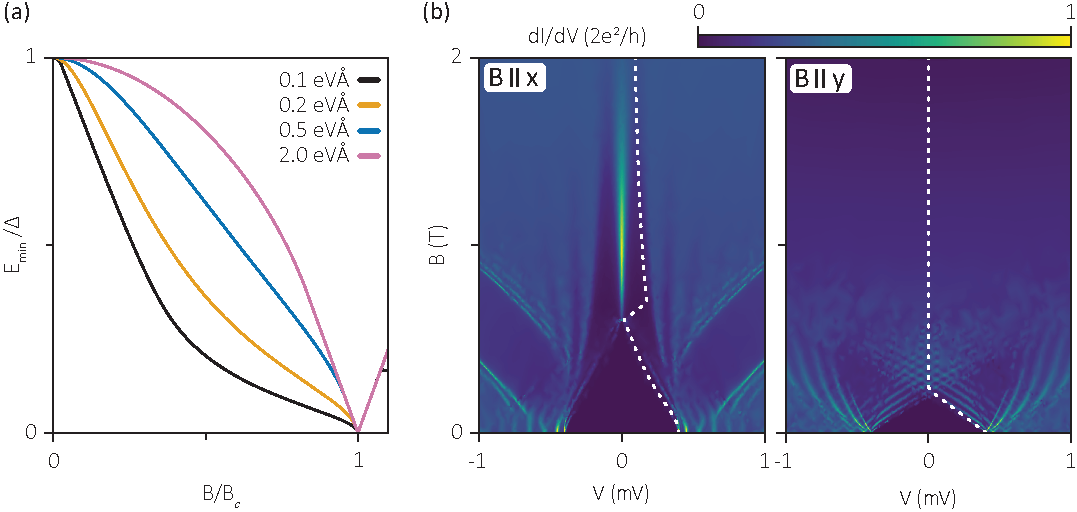
\includegraphics[width=0.95\textwidth]{chapter_spinorbit/figures/SFig7_AlphaFitting.pdf}
\caption{\label{fig:SOIFit}
Extracting SOI strength from gap closing curvature.
(a) Lowest energy state $E_{\mathrm{min}}$ determining the gap in the one-dimensional model given by equation S1 as a function of magnetic field, $B$, in units of the critical field $B_c=\sqrt{\Delta^2+\mu^2}$ for various spin-orbit strengths $\alpha$.
The curvature of the gap closing is strongly affected by $\alpha$.
Stronger SOI counteracts the Zeeman effect up to larger $B/B_c$, leading initially to a slow gap closing, followed by a sharp gap closing when approaching the critical field, where the lowest energy state is at $k \approx 0$ for which $B_{\mathrm{SO}}(k)$ vanishes.
The remaining parameters are: $\Delta(0)$ = 1 meV, $\mu$ = 2 meV.
(b) Comparison of the numerical simulations on the 3D tight binding model, including the orbital effect (color map), with the 1D model given by equations (S1) and (S2) which does not account for the orbital effect (dashed lines).
By adjusting the $g$-factor used in the Majorana nanowire model from $g$ = 50 to 65 to match the gap closing for $B \parallel B_{\mathrm{SO}}$, keeping all other parameters the same in both models, we find good agreement for the gap closing for $B \parallel x$.
We use this same approach to take the orbital effect into account in an effective manner in fits of the experimentally observed gap closing.
The remaining parameters used in the simulations shown here are $\Delta(0)$ = 0.45 meV, $\mu$ = 0.95 meV, $\alpha$ = 0.2 eV\AA, $\Delta V_G$ = -10 meV.
}
\end{figure}

\subsubsection{Estimation of SOI strength based on level repulsion}
SOI induces coupling between states of different momentum and spin in finite length Majorana nanowires, which leads to level repulsion when energy levels are nearly degenerate \cite{Stanescu2013}.
Recently this level repulsion between longitudinal states within the same subband was used to estimate a SOI strength in epitaxial Al-InSb nanowires \cite{DeMoor2018}.
Here, we follow the same procedure to estimate the SOI strength in a seperate device with a NbTiN superconductor that exhibits such level repulsion.
We consider a low energy model of two levels dispersing in the magnetic field due to the Zeeman effect, coupled to each other by SOI with the matrix element $\delta_{\mathrm{SO}}$:

\begin{equation}
H = \begin{bmatrix}
E_0 + \frac{1}{2}g_0 \mu_B B & \delta_{\mathrm{SO}} \\
\delta_{\mathrm{SO}} & E_1 - \frac{1}{2}g_1 \mu_B B
\end{bmatrix}
\end{equation}

We fit the eigenenergies of $H$ to our experimental data [Fig.~\ref{fig:SOIlevelrep}a] to extract $\delta_{\mathrm{SO}}$.
The precise value of the coupling parameter $\delta_{\mathrm{SO}}$ depends not only on $\alpha$, but also on the details of the confinement and on the coupling strength to the superconductor \cite{DeMoor2018}.
A rough estimate, with reasonable agreement to numerical simulations, was proposed to be: $2\delta_{\mathrm{SO}}$ = $\alpha \pi/ L$, where $L$ is the length of the wire.
The extracted $\delta_{\mathrm{SO}}$ is shown in Fig.~\ref{fig:SOIlevelrep}(b) for various values of the super gate voltage $V_{\mathrm{SG}}$.
As $V_{\mathrm{SG}}$ becomes more negative, we see an increase in $\delta_{\mathrm{SO}}$, consistent with an increasing electric field in the nanowire.
We can estimate $\alpha \sim$ 0.4 -- 0.55 eV\AA.
Considering the uncertainty in the relation between $\alpha$ and $\delta_{\mathrm{SO}}$ and variation in the electrostatic environment of different devices, this magnitude is in line with our estimation based on the gap closing curvature.

\begin{figure}[h]
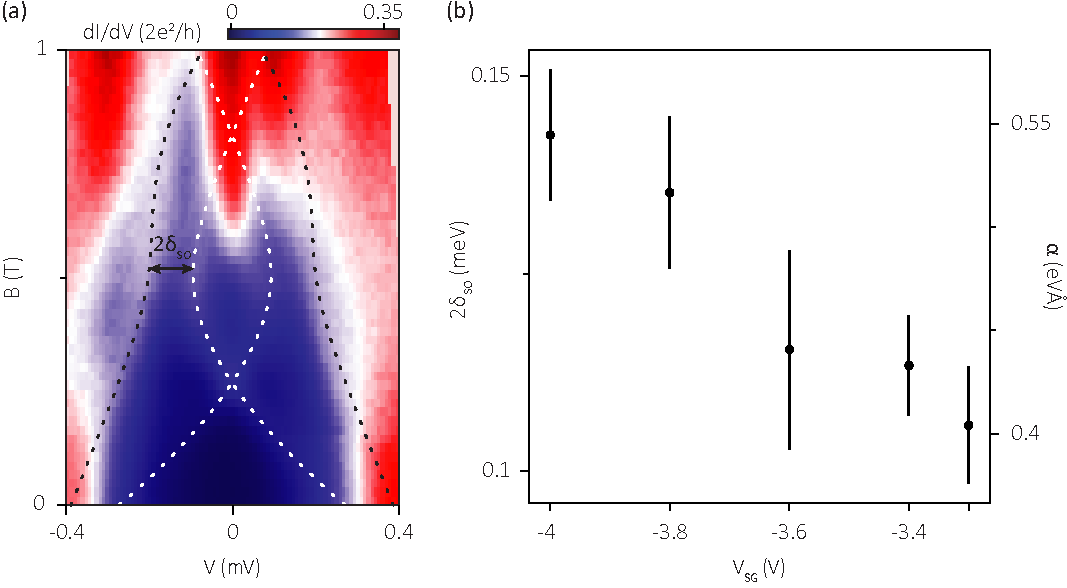
\includegraphics[width=0.95\textwidth]{chapter_spinorbit/figures/SFig3_Anticrossing.pdf}
\caption{\label{fig:SOIlevelrep}
Extracting the SOI strength from level repulsion.
(a) $dI/dV$ as a function of $V$ and $B$ at $V_{\mathrm{SG}}$ = -3.3 V, measured in device E.
Two Andreev states come down from the gap edge and exhibit an avoided crossing around $B = 0.5$ T.
The dashed lines indicate fits to the solution of equation (S3).
The extracted coupling $\delta_{\mathrm{SO}}$ between the Andreev levels is indicated by the arrow.
(b) $2\delta_{\mathrm{SO}}$ as a function of $V_{\mathrm{SG}}$.
The right axis shows the estimation of the SOI strength using $\alpha = 2\delta_{\mathrm{SO}}L/\pi$ for the 1.2 $\mu$m long superconducting region.
The errorbars show the standard deviation in $\delta_{\mathrm{SO}}$ obtained from the fits.
}
\end{figure}

\clearpage
\subsection{Supplemental Experimental Data}
\begin{figure}[h!]
\centering
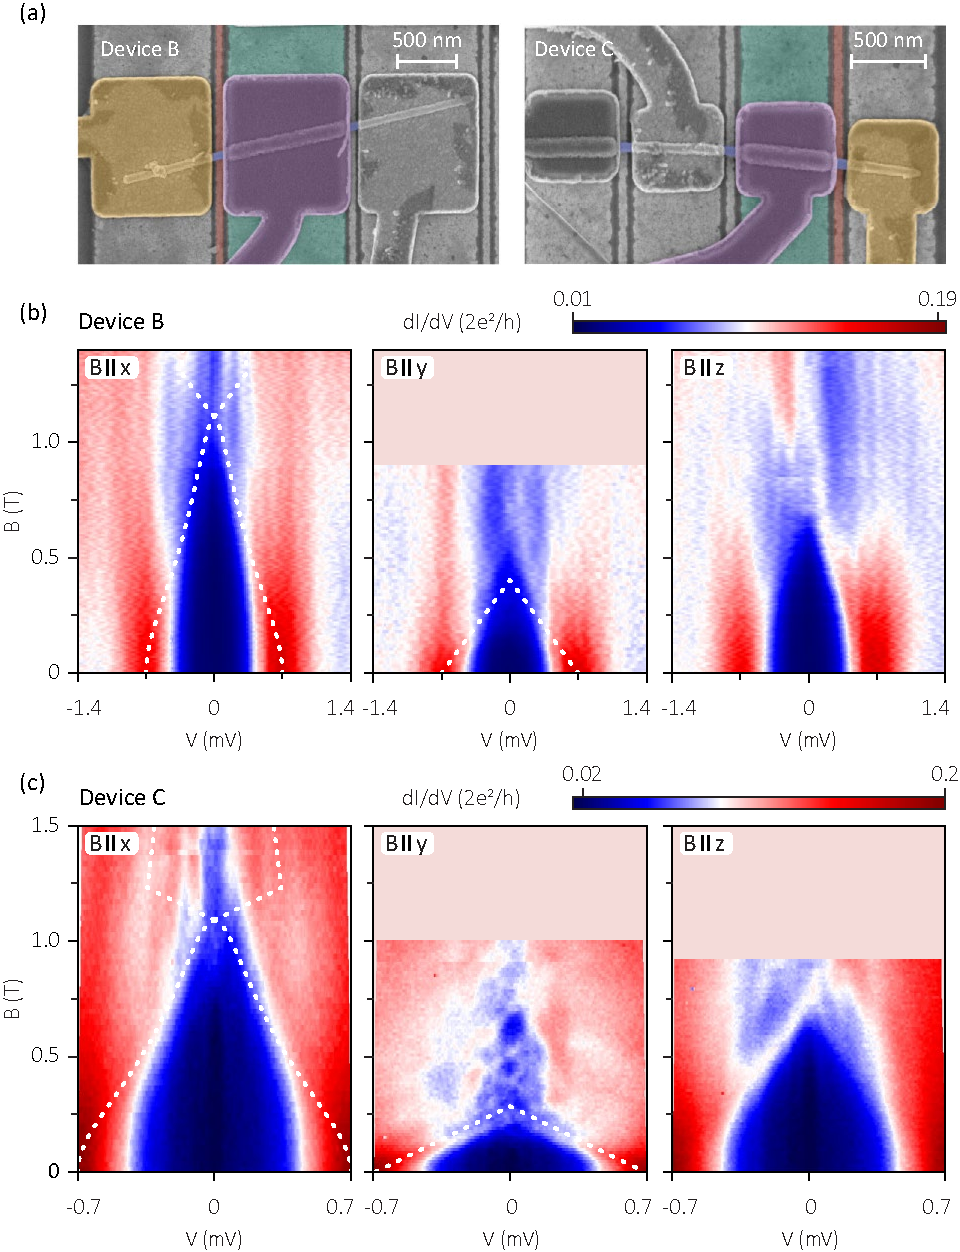
\includegraphics[width=0.77\textwidth]{chapter_spinorbit/figures/SFig1_Bsweeps_reproduced.pdf}
\caption{\label{fig:BsweepsReproduced}
Anisotropic gap closing in additional devices.
(a) False colored scanning electron micrographs of additional devices B (used in Fig.~3) and C, showing anisotropy similar to the device in Fig.~1(e).
(b,c) Differential conductance, $dI/dV$, as a function of the magnetic field, $B$, along the $x$, $y$, and $z$-axes (from left to right).
The gap closes at much lower fields along the $y$-axis than the $x$ and $z$-axes in all devices fully covered with the superconductor.
The white dashed lines indicate fits to the gap closing from which we extract a spin-orbit strength $\alpha$ of 0.3 $\pm$ 0.1 eV\AA\ [for (b)] and 0.35 $\pm$ 0.05 eV\AA\ [for (c)], with $g$ = 60, 85 and $\mu$ = 1.8, 2.7 meV as the remaining fit parameters for (b), (c) respectively.
We note that we do not observe clear reopening of the gap in all devices, which theoretical studies have attributed to the negligible contribution to the tunneling conductance of the states associated with the gap reopening due to their spatial wave function extension into the middle of the wire leading to minimal weight near the tunnel barrier \cite{Prada2012,Pientka2012,Stanescu2012,Liu2019}.
The super gate was set to $V_{\mathrm{SG}}$ = -1.5 V, -2.6 V in (b), (c) respectively.
}
\end{figure}

\begin{figure}[p!]
\centering
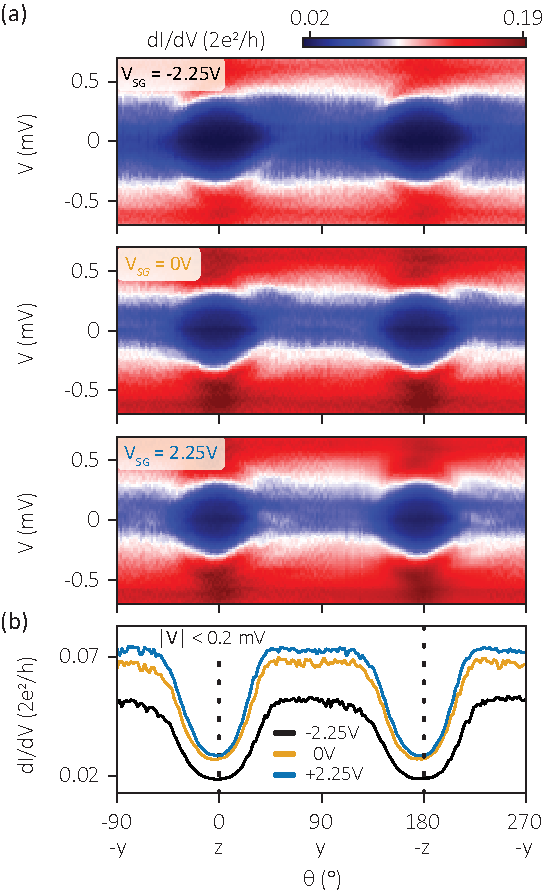
\includegraphics[width=0.55\textwidth]{chapter_spinorbit/figures/SFig4_YZrot_Full1_reproduced.pdf}
\caption{\label{fig:YZrotRep}
Gap dependence on magnetic field orientation in \textit{zy}-plane in device A.
(a) Differential conductance, $dI/dV$, as a function of bias voltage, $V$, upon rotation of the magnetic field at 0.25 T over angles $\Theta$ between $z$ and $y$ with different voltages on the super gate $V_{\mathrm{SG}}$ in the three panels.
This is the same device as presented in Fig.
1 (b) Horizontal line cuts of (a) averaged over a bias range $|V| < 0.2$ mV, showing that the hardest gap is at $\Theta = 0$, and increased $V_{\mathrm{SG}}$ suppresses the gap when $B$ is along $y$, the same behaviors observed in device B [Fig.~3].
}
\end{figure}

\begin{figure}[p!]
\centering
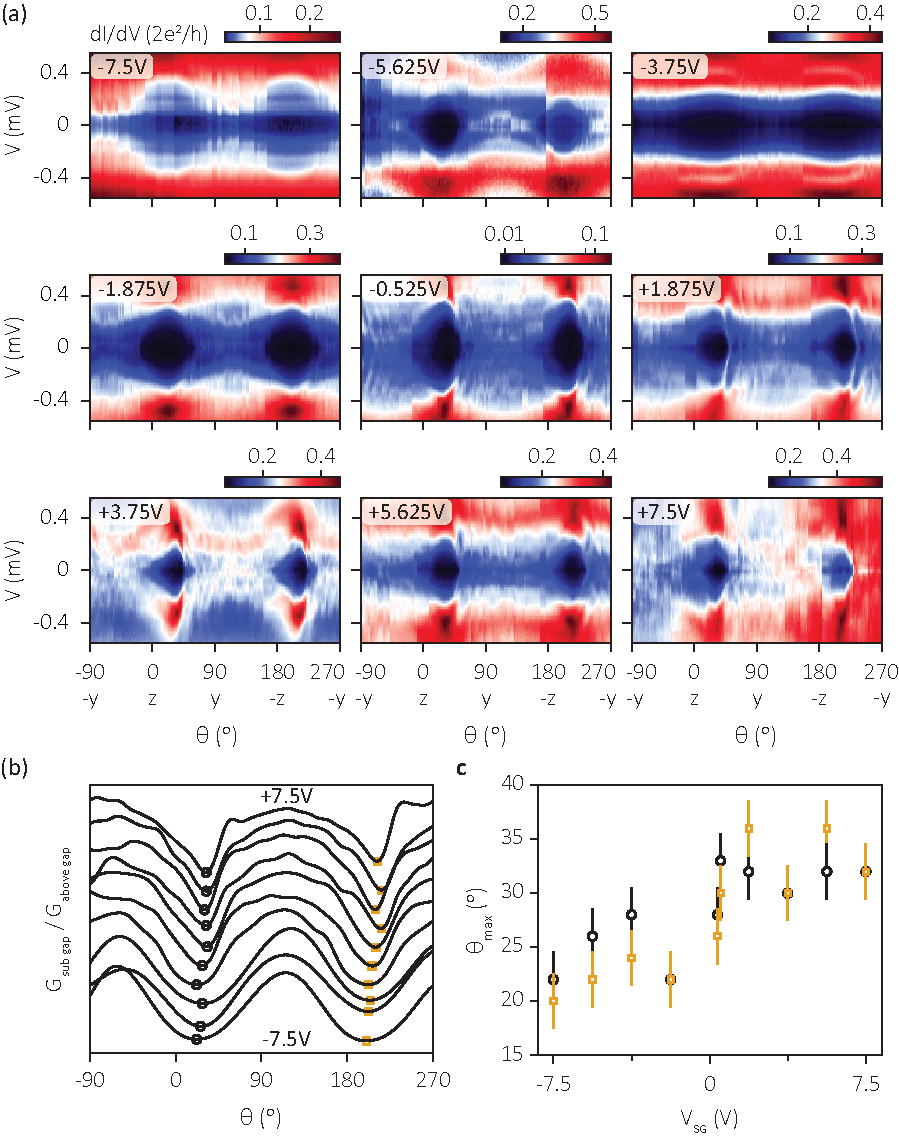
\includegraphics[width=0.85\textwidth]{chapter_spinorbit/figures/SFig5_SGdep_half_updated.pdf}
\caption{\label{fig:SGdep}
Dependence of spin-orbit direction on super gate voltage in device D, which is partially covered by NbTiN.
(a) Differential conductance, $dI/dV$, as a function of bias voltage, $V$, and angle $\Theta$ between $z$ and $y$ at various values of $V_{\mathrm{SG}}$ as indicated in the insets.
The data is measured at slightly different field magnitudes between 0.1 and 0.2 T for the different $V_{\mathrm{SG}}$ to optimize the anisotropy between $y$ and $z$.
The discontinuities in $dI/dV$ that are visible for some of the scans are likely caused by charge fluctuations in the dielectric environment.
(b) The ratio between the sub gap conductance (averaged over $|V| < 0.2$ V) and the above gap conductance (averaged over $|V| > 0.4$ V) with $V_{\mathrm{SG}}$ increasing from bottom to top and offset for clarity.
The minima of the curves signify the angle at which the gap is hardest, $\Theta_{\mathrm{max}}$, which shifts to higher angles at increasing $V_{\mathrm{SG}}$.
A lowpass filter is applied along the $\Theta$ direction to suppress the effect of the charge instabilities (this procedure does not affect the minima for the measurements without charge instabilities, such as in Fig.~4).
(c) $\Theta_{\mathrm{max}}$ as determined from the first (black) and second (yellow) minimum of the curves in (b) as a function of $V_{\mathrm{SG}}$.
The second minima (yellow) signify $\Theta_{\mathrm{max}}$ at negative $B$ and are subtracted by \ang{180} accordingly.
}
\end{figure}

\begin{figure}[p!]
\centering
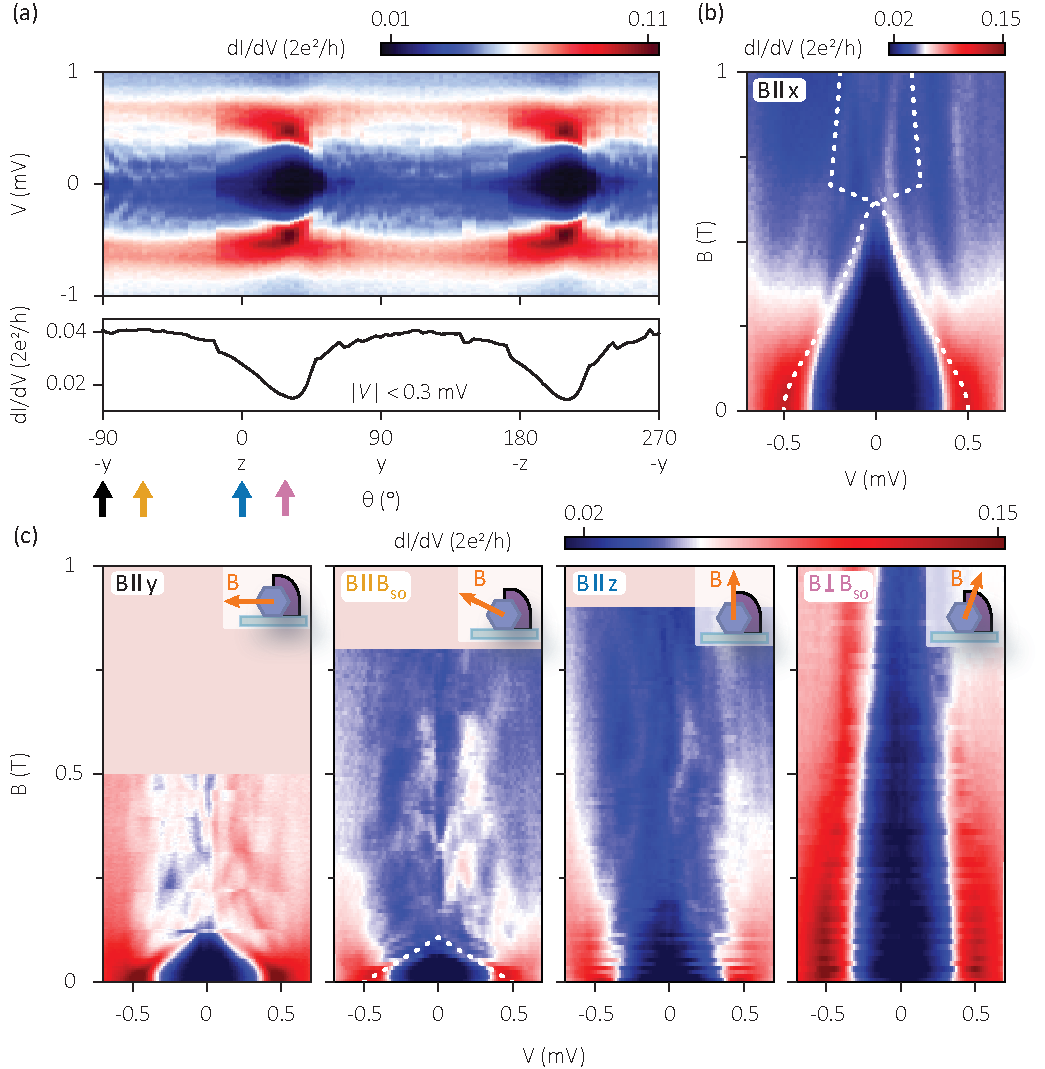
\includegraphics[width=0.95\textwidth]{chapter_spinorbit/figures/SFig6_Bsweeps_half.pdf}
\caption{\label{fig:BsweepsHalf}
Gap dependence on magnetic field orientation in device E, which is partially covered by NbTiN.
(a) Differential conductance, $dI/dV$, as a function of the angle $\Theta$ between the $z$ and $y$-axes at $V_{\mathrm{SG}}$ = 0.525 V and $B$ = 0.1 T, with a horizontal line cut averaged over a bias range $|V| < 0.3$ mV in the lower panel.
(b) $dI/dV$ as a function of the magnetic field $B$ along the nanowire axis, with the white dashed lines showing the fit to the gap closing, resulting in a spin-orbit strength $\alpha$ of 0.35 $\pm$ 0.05 eV\AA\ (the other fit parameters are $g$ = 160, see $B \parallel B_{\mathrm{SO}}$ in (c), and $\mu$ = 2.8 meV).
(c) $dI/dV$ as a function of $B$ along $y$, $B_{\mathrm{SO}}$, $z$ and perpendicular to $B_{\mathrm{SO}}$ from left to right, with the colors in the headers corresponding to the colored arrows in (a).
The illustrations in the insets indicate the direction of the magnetic field.
Note that due to the changed orientation of $B_{\mathrm{SO}}$, $B$-sweeps along directions rotated by $\sim$\ang{25} from the $y$-axis (second panel, $B \parallel B_{\mathrm{SO}}$) and the $z$-axis (right panel, $B \perp B_{\mathrm{SO}})$  now exhibit strong anisotropy, instead of the $y$ and $z$-axes which show strong anisotropy in devices symmetrically covered by NbTiN.
}
\end{figure}

\references{dissertation}
